\section{The audit of the final tuned world models}
\label{sec:tuned}

The audit read the world model the companion paper~\cite{rwm} reports for each
of its \tSets{} data sets: six Dominick's categories, Frat, M5 and Favorita, each
the average of five copies fitted with different seeds (one copy on M5), with
one saved model per rolling window, \tWindows{} windows in all. No model was
refitted or tuned for the audit, and no audit result changed a setting. The
checks and their thresholds are those fixed before the first audit
(Table~\ref{tab:thresholds}); Table~\ref{tab:tunedpass} and
Figure~\ref{fig:tunedchecks} give the results.

\textbf{The tuned models' explanations add up, depend on what was learned and
carry the plan in their state, but on most data sets a deeper price cut can lower
the forecast, and both models state a larger price response than the one
measured.}

\begin{table*}[t]\centering
\caption{\textbf{The explanations add up under the model's own plan on every
window; C4 fails on every data set but Frat.} Share of windows passing each
check, \%, for the final tuned world model of each data set. C1 is scored under
the audit's plan for nothing planned (as fixed) and under the model's own (as
amended); C3 is the rank agreement of lifts between the model's five copies (n/a
on M5, whose final model is one copy); C6 the rank agreement of total lift with
the data set's final tuned LightGBM. Thresholds in Table~\ref{tab:thresholds}.}
\label{tab:tunedpass}
\footnotesize\setlength{\tabcolsep}{6pt}\begin{tabular}{@{}lrrrrrrrr@{}}
\toprule
Data & Windows & C1 (audit plan) & C1 (own plan) & C2 & C3 & C4 & C5 & C6 \\
\midrule
Analgesics & 6 & 0 & 100 & 83 & 83 & 0 & 83 & 0 \\
Bottled juice & 6 & 17 & 100 & 33 & 100 & 0 & 83 & 33 \\
Cheese & 6 & 0 & 100 & 100 & 100 & 0 & 83 & 17 \\
Frozen entrees & 6 & 0 & 100 & 83 & 83 & 0 & 83 & 83 \\
Soft drinks & 6 & 0 & 100 & 100 & 100 & 0 & 67 & 67 \\
Snacks & 6 & 0 & 100 & 83 & 100 & 0 & 67 & 33 \\
Frat & 4 & 0 & 100 & 50 & 100 & 100 & 100 & 100 \\
M5 & 4 & 0 & 100 & 100 & 0 & 0 & 0 & 0 \\
Favorita & 4 & 100 & 100 & 100 & 75 & 0 & 100 & 0 \\
\bottomrule
\end{tabular}
\end{table*}

\begin{figure*}[t]\centering
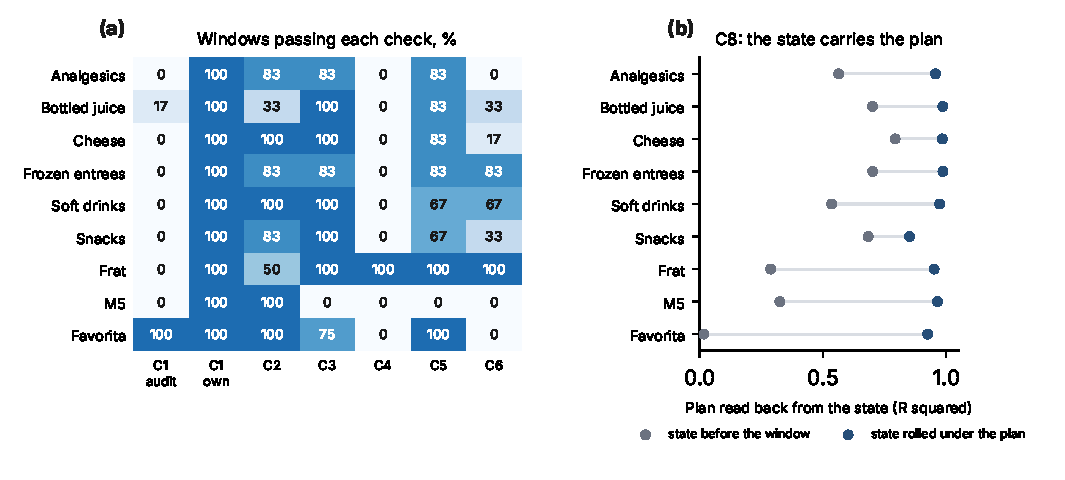
\includegraphics[width=\textwidth]{figs/fig_tuned_checks.pdf}
\caption{\textbf{The state rolled under the plan carries the plan on every data
set.} \textbf{(a)} Share of windows passing each check (Table~\ref{tab:tunedpass}).
\textbf{(b)} C8: how well the plan inputs of each period can be read back from
the world model's state, from the state before the window and from the state
rolled forward under the plan (the gain is what the rolled state adds).}
\label{fig:tunedchecks}
\end{figure*}

\paragraph{C1: the parts add up under the model's own plan}
Under the model's own plan for nothing planned, every window of all \tSets{}
data sets passes C1. Under the audit's plan, \tCOneMean\% of windows pass; as in
the earlier audit (Section~\ref{sec:results}), every failure sits where the
audit's plan differs from the model's own regular price, not in how the parts
add up.

\paragraph{C2 and C3: the lifts depend on what was learned, and the copies agree}
Randomising the learned lift readout changes the lifts on \tCTwoMean\% of
windows (C2). The five copies of each model rank item lifts alike: the rank
agreement between copies is \tCThreeLo{} to \tCThreeHi{}, and \tCThreeMean\% of
windows pass C3.

\paragraph{C4: on most data sets a deeper cut can lower the forecast}
C4 fails on every data set but Frat. A deeper price cut lowers the forecast for
\tCFourDomLo{} to \tCFourDomHi\% of items on the Dominick's categories,
\tCFourFav\% on Favorita and \tCFourMfive\% on M5, against \tCFourFrat\% on Frat.
The forecast is accurate on these data sets (paper~1), so this is a fault in how
the model responds to price depth, not in its forecasts of the plans it saw.

\paragraph{C5 and C6: agreement with sales and with LightGBM}
The forecasts in planned weeks match sales in level and order on \tCFiveMean\%
of windows (C5); M5 fails, ranking planned weeks with a correlation of
\tCFiveRankMfive{} against the 0.3 required. The world model and the tuned
LightGBM agree on which items gain most from the plan with a rank correlation of
\tCSixLo{} to \tCSixHi{}; \tCSixMean\% of windows reach the 0.5 required (C6).

\paragraph{C7: both models state a larger price response than the one measured}
On the 38 scored zone episodes (Section~\ref{sec:zones}), the measured pooled
slope of category units on price is \tSlopeMeas{} (95\% interval \tSlopeMeasLo{}
to \tSlopeMeasHi{}). The world model states \tSlopeWm{} (\tSlopeWmLo{} to
\tSlopeWmHi{}) and LightGBM \tSlopeLgb{} (\tSlopeLgbLo{} to \tSlopeLgbHi{})
(Figure~\ref{fig:tunedc7}). Both state a response about twice the measured one,
the world model slightly more than LightGBM.

\begin{figure*}[t]\centering
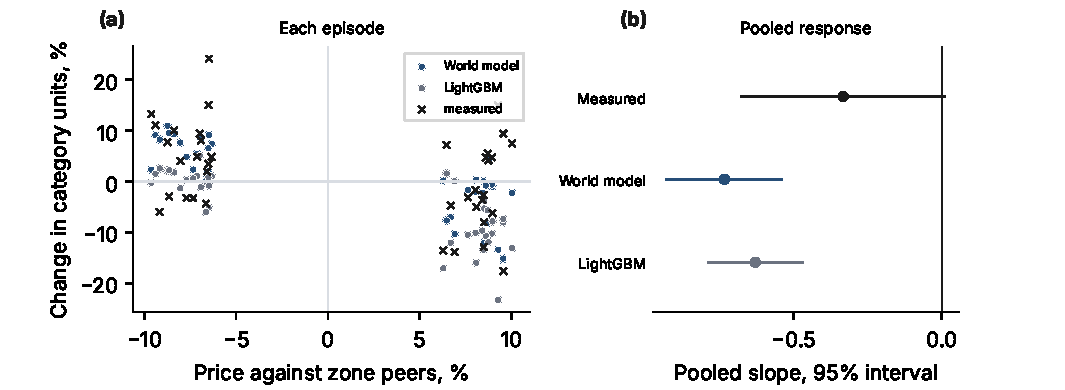
\includegraphics[width=\textwidth]{figs/fig_tuned_c7.pdf}
\caption{\textbf{Both tuned models state a larger price response than the one
measured.} \textbf{(a)} For each scored zone episode, the change in category
units the world model and LightGBM state for the price deviation, and the change
measured. \textbf{(b)} Pooled slopes with 95\% intervals.}
\label{fig:tunedc7}
\end{figure*}

\paragraph{C8: the state carries the plan}
The plan inputs of each period can be read back from the state rolled forward
under the plan with $R^2$ of \tReadRolledLo{} to \tReadRolledHi{}, and rolling the
state forward adds \tReadGainLo{} to \tReadGainHi{} to what the state before the
window holds (Figure~\ref{fig:tunedchecks}b). The model's state is where it
keeps the plan, as a world model should.

\paragraph{Checks against accuracy: no link across the searches' versions}
Across the \tSearchVersions{} model versions the settings searches saved
(\tConfigsAll{} configurations, each scored on the same data and windows as the
others of its search), the number of checks a configuration passed was not
related to its accuracy: the pooled rank correlation with item-by-store error is
\tRhoAll{} (95\% interval \tRhoAllLo{} to \tRhoAllHi{}, $p=\tPAll$), and
\tRhoNoOneFive{} ($p=\tPNoOneFive$) leaving out C1 and C5. Tuning for accuracy
did not make the explanations better or worse.
